\documentclass[a4paper]{article}

\usepackage[utf8x]{inputenc}    
\usepackage[T1]{fontenc}
\usepackage[spanish]{babel}
\usepackage{multicol}

\usepackage{wrapfig}
\usepackage{graphicx}

\usepackage{bm}
\usepackage{amsxtra} 
\usepackage{amssymb}% to get the \mathbb alphabet
\usepackage{amsmath}

\usepackage[spanish]{cleveref}


\usepackage[box,completemulti,separateanswersheet]{automultiplechoice}    
\def\AMCformQuestion#1{\vspace{\AMCformVSpace}\par {\sc Pregunta #1:} }    
\def\AMCbeginQuestion#1#2{\par\noindent{\bf Pregunta #1}#2\hspace*{1em}}
\def\AMCcleardoublepage{\ifodd\thepage\clearpage\mbox{}\fi\clearpage}

\begin{document}

\AMCrandomseed{1237893}

%%%%%%%%%%%%%%%%%%%%%%%%%%%%%%%%%%%%%%%%%%%%%%%%%%%%%%%%%%%%%%%%%%%%%%%%%%%%%
\element{test1}{
\begin{question}{p1}
El valor del desplazamiento en direcci\'on $x$ del punto I vale aprox:
\begin{multicols}{2}
\begin{choices}
	\correctchoice{$1.5$ cm}
	\wrongchoice{$11.7$ cm}
	\wrongchoice{$0.63$ cm}
	\wrongchoice{$5.9$ cm}
\end{choices}
\end{multicols}
\end{question}
}
%%%%%%%%%%%%%%%%%%%%%%%%%%%%%%%%%%%%%%%%%%%%%%%%%%%%%%%%%%%%%%%%%%%%%%%%%%%%%
\element{test1}{
\begin{question}{p2}
El valor del giro en direcci\'on $z$ del punto C vale aprox:
\begin{multicols}{2}
\begin{choices}
	\correctchoice{$-2.5\cdot10^{-3}$ rad}
	\wrongchoice{$-1.1\cdot10^{-4}$ rad}
	\wrongchoice{$-5.6\cdot10^{-3}$ rad}
	\wrongchoice{$2.1\cdot10^{-4}$ rad}
\end{choices}
\end{multicols}
\end{question}
}
%%%%%%%%%%%%%%%%%%%%%%%%%%%%%%%%%%%%%%%%%%%%%%%%%%%%%%%%%%%%%%%%%%%%%%%%%%%%%
\element{test1}{
\begin{question}{p3}
El valor de la máxima flecha vertical en el vano CF vale aprox.:
\begin{multicols}{2}
\begin{choices}
	\correctchoice{$3.4$ mm}
	\wrongchoice{$2.1$ mm}
	\wrongchoice{$0.91$ mm}
	\wrongchoice{$1.7$ mm}
\end{choices}
\end{multicols}
\end{question}
}
%%%%%%%%%%%%%%%%%%%%%%%%%%%%%%%%%%%%%%%%%%%%%%%%%%%%%%%%%%%%%%%%%%%%%%%%%%%%%
\element{test1}{
\begin{question}{p4}
El valor de la componente vertical de la reacción en el apoyo de la columna central vale aprox.:
\begin{multicols}{2}
\begin{choices}
	\correctchoice{$620.9$ kN}
	\wrongchoice{$ 120.4$ kN}
	\wrongchoice{$ 53.1$ kN}
	\wrongchoice{$ 8001.3$ kN}
\end{choices}
\end{multicols}
\end{question}
}
%%%%%%%%%%%%%%%%%%%%%%%%%%%%%%%%%%%%%%%%%%%%%%%%%%%%%%%%%%%%%%%%%%%%%%%%%%%%%
\element{test1}{
\begin{question}{p4b}
El valor de la componente horizontal de la reacción en el apoyo izquierdo vale aprox.:
\begin{multicols}{2}
\begin{choices}
	\correctchoice{$-29.0$ kN}
	\wrongchoice{$ -12.4$ kN}
	\wrongchoice{$ 93.1$ kN}
	\wrongchoice{$ -8.90$ kN}
\end{choices}
\end{multicols}
\end{question}
}
%%%%%%%%%%%%%%%%%%%%%%%%%%%%%%%%%%%%%%%%%%%%%%%%%%%%%%%%%%%%%%%%%%%%%%%%%%%%%
\element{test1}{
\begin{question}{p5}
El valor del momento máximo en direcci\'on $z$ en el centro del vano FI, en valor absoluto, vale aprox.:
\begin{multicols}{2}
\begin{choices}
	\correctchoice{$ 73.3$ kN m}
	\wrongchoice{$34.1$ kN m}
	\wrongchoice{$51.9$ kN m}
	\wrongchoice{$104.9$ kN m}
\end{choices}
\end{multicols}
\end{question}
}
%%%%%%%%%%%%%%%%%%%%%%%%%%%%%%%%%%%%%%%%%%%%%%%%%%%%%%%%%%%%%%%%%%%%%%%%%%%%%
%\element{test1}{
%\begin{question}{p6}
%El valor del cortante máximo en el vano FI, en valor absoluto, vale aprox.:
%\begin{multicols}{2}
%\begin{choices}
%	\correctchoice{$ 46$ kN}
%	\wrongchoice{$ 21 $ kN}
%	\wrongchoice{$  12$ kN}
%	\wrongchoice{$  108$ kN}
%\end{choices}
%\end{multicols}
%\end{question}
%}
%%%%%%%%%%%%%%%%%%%%%%%%%%%%%%%%%%%%%%%%%%%%%%%%%%%%%%%%%%%%%%%%%%%%%%%%%%%%% 
\element{test1}{
\begin{question}{p7}
El valor del axil máximo en el vano FI, en valor absoluto, vale aprox.:
\begin{multicols}{2}
\begin{choices}
	\correctchoice{$ 359$ kN}
	\wrongchoice{$ 30 $ kN}
	\wrongchoice{$  1140$ kN}
	\wrongchoice{$  880$ kN}
\end{choices}
\end{multicols}
\end{question}
}
%%%%%%%%%%%%%%%%%%%%%%%%%%%%%%%%%%%%%%%%%%%%%%%%%%%%%%%%%%%%%%%%%%%%%%%%%%%%%
\element{test1}{
\begin{question}{p8}
En la formulación de vigas de Timoshenko, el esfuerzo cortante:
%\begin{multicols}{2}
\begin{choices}
       \wrongchoice{Sólo se puede calcular con la ecuación de equilibrio de momentos
       ya que no interviene en las ecuaciones constitutivas}
        \correctchoice{Se calcula a partir de la deformación angular $\gamma_{xz}$}
        \wrongchoice{Por hipótesis, se toma iguaL a $0$}
        \wrongchoice{Ninguna de las otras respuestas es correcta}
\end{choices}
%\end{multicols}
\end{question}
}
%%%%%%%%%%%%%%%%%%%%%%%%%%%%%%%%%%%%%%%%%%%%%%%%%%%%%%%%%%%%%%%%%%%%%%%%%%%%%%
\element{test1}{
\begin{question}{p9}
Los elementos finitos de viga de Bernoulli:
\begin{choices}
        \correctchoice{No consideran la deformación por esfuerzo cortante}
        \wrongchoice{Incorporan la hipótesis de que las secciones normales a la directriz pueden deformarse}
        \wrongchoice{Las funciones de interpolación de los elementos finitos \(N_a(x)\) necesariamente son cuadráticas}
        \wrongchoice{Las funciones de interpolación de los elementos finitos \(N_a(x)\) pueden ser lineales}
\end{choices}
\end{question}
}
%%%%%%%%%%%%%%%%%%%%%%%%%%%%%%%%%%%%%%%%%%%%%%%%%%%%%%%%%%%%%%%%%%%%%%%%%%%%%%
\element{test1}{
\begin{question}{p10}
Una oficina de ingeniería presenta un informe de un cálculo de elementos finitos
realizado con elementos triangulares de deformación constante (triángulo isoparamétrico de tres nodos). Esos cálculos sólo son admisibles si:
\begin{choices}
        \correctchoice{Están referidos a un problema lineal de conducción de calor}
        \wrongchoice{Están referidos a la respuesta un material elástico lineal incompresible}
        \wrongchoice{Están referidos a la respuesta mecánica lineal  de una estructura que trabaja
        a flexión}
        \wrongchoice{Están referidos al análisis de una estructura laminar no lineal}
\end{choices}
\end{question}
}
%%%%%%%%%%%%%%%%%%%%%%%%%%%%%%%%%%%%%%%%%%%%%

\scoringDefaultS{b=1,m=-1/(N-1)}

\onecopy{10}{    

%%% beginning of the test sheet header:    

\noindent{\large\bf Método de los Elementos Finitos  \hfill MUECYM \hfill FINAL ORD. \# Ej. 2}
\begin{center}
%\vspace*{.1cm}
%Se atribuirá puntuación negativa a las respuestas incorrectas.\\
\vspace*{.1cm}
20 ene 2025. \hspace{7cm} Tiempo: 45 minutos.\\


\end{center}

\vspace{1ex}

El pórtico de dos vanos mostrado en la figura es de hormigón armado con módulo de elasticidad $E=32$ GPa, coeficiente de Poisson $\nu=0.20$, y densidad de masa  $\rho=2548.42$ kg/m$^3$. Las secciones de las vigas son de $0.30$ m $\times$ $0.60$ m (base y altura), y las columnas tienen sección cuadrada de $0.40$ m de lado. Las cargas actuantes sobre la estructura son el peso propio del pórtico, dos cargas puntuales verticales (en J y K), una carga puntual horizontal (en C) y una carga distribuida (sobre las vigas). Los apoyos A, D y G se consideran perfectamente empotrados. Los letras B, J, E, K y H indican la mitad de cada uno de los respectivos elementos estructurales.

Se pide realizar un modelo de vigas con elementos tipo B23, tamaño de elementos $0.5$ m y responder las preguntas del cuestionario.

Las longitudes del pórtico son tal como sigue: $l_{1}= 6$ m, $l_{2}= 5$ m, $l_{3}= 3$ m, $l_{4}$ y $l_{5}= 5$ m. Las cargas son $V_{1}= 70$ kN, $V_{2}= 50$ kN, $H_{1}= 488.40$ kN, y $q_{1}= 100$ kN/m. Las dimensiones de los elementos estructurales son $a= 0.40$ m, $b= 0.30$ m y $c= 0.60$ m.
\\
%\begin{center}
%	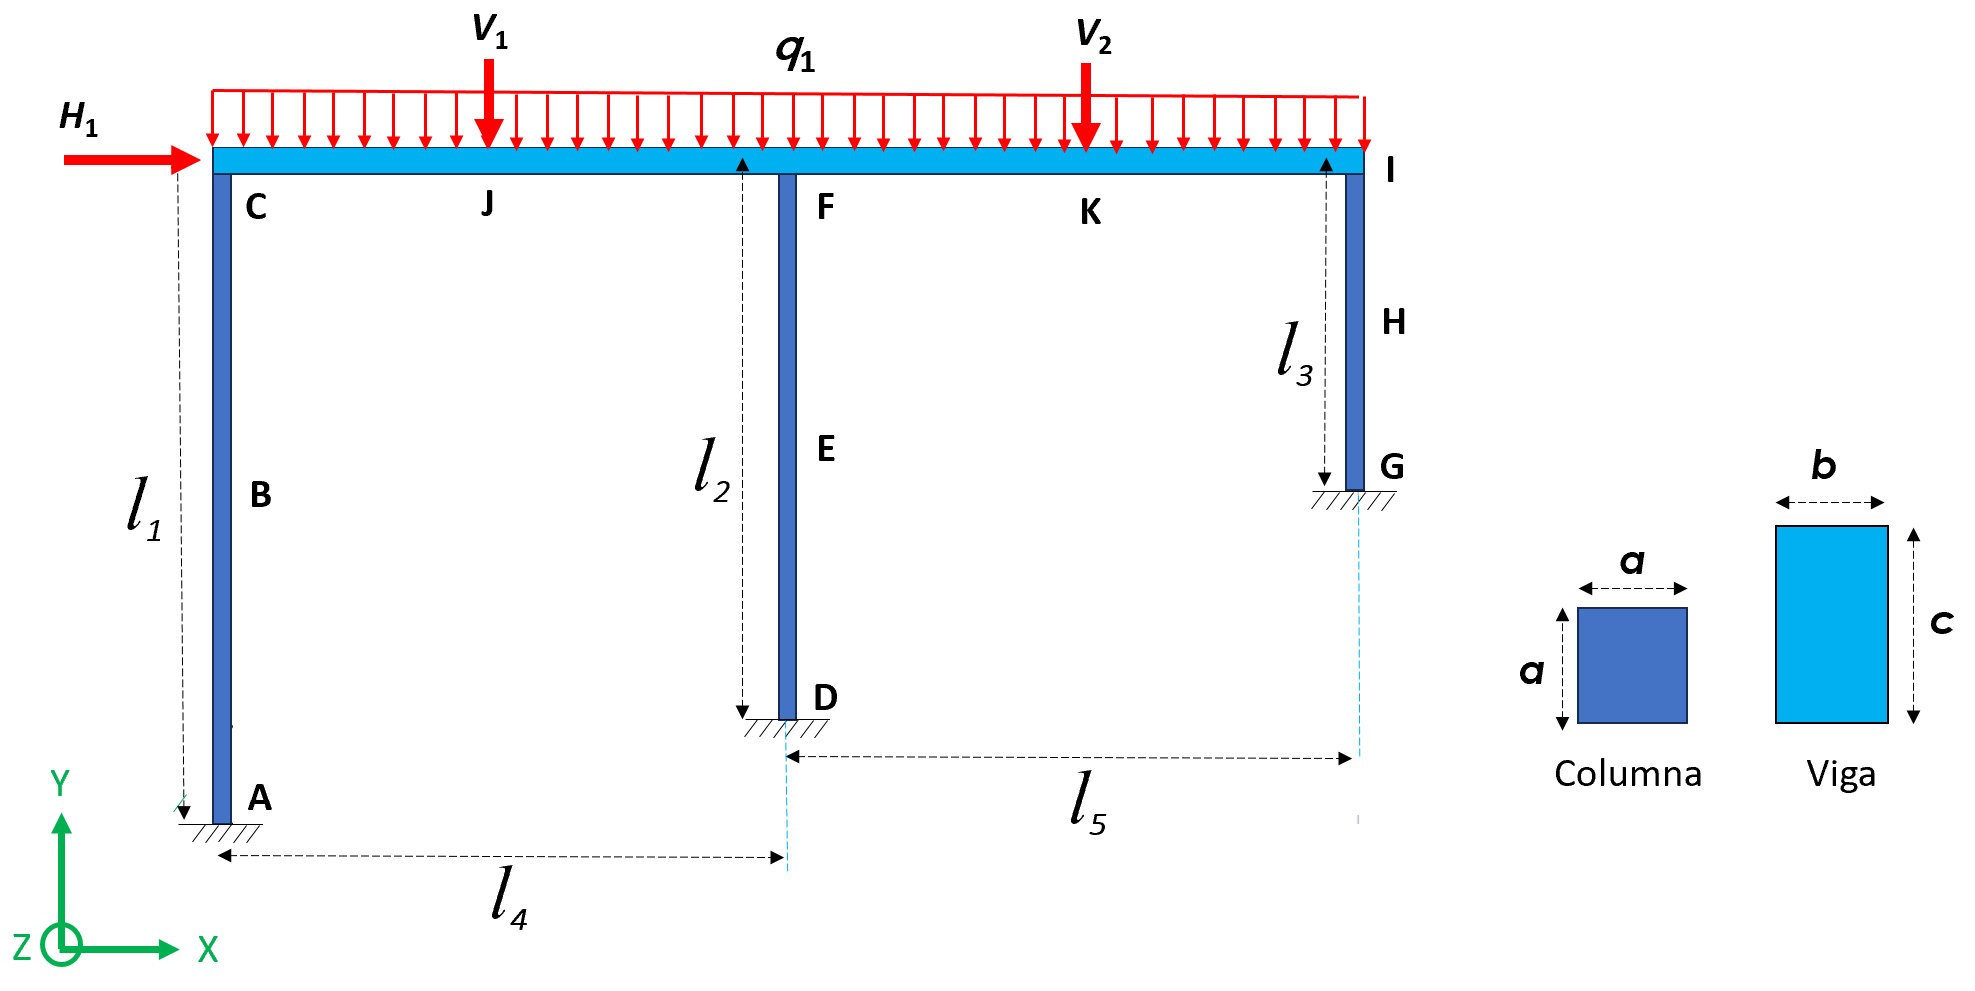
\includegraphics[width=1.05\textwidth]{figuraNT2023}
%\end{center}


\hrulefill
\vspace{4mm}

%%% end of the header

\shufflegroup{test1}
\insertgroup{test1}

%\AMCcleardoublepage    
\clearpage

\AMCformBegin    

%%% beginning of the answer sheet header

\noindent\AMCcode{nummat}{2}\hspace*{\fill}
\begin{minipage}{.7\linewidth}
$\longleftarrow{}$ Escriba su número de matrícula marcando los dígitos
en los recuadros (con ceros a la izquierda si el número es de menos de dos dígitos) y el nombre y apellidos debajo.

\vspace{3ex}

\namefield{\fbox{
   \begin{minipage}{.9\linewidth}
     Apellidos, Nombre:

     \vspace*{.5cm}\dotfill
     \vspace*{1mm}
   \end{minipage}
 }}
\end{minipage}

\begin{center}
 \bf\em Debe dar las respuestas exclusivamente en esta hoja (las respuestas en las demás hojas no serán tenidas en cuenta).
\end{center}

%%% end of the answer sheet header


\AMCform    

\AMCcleardoublepage    

}  

\end{document}
